\documentclass[tikz,border=3pt]{standalone}

\usepackage[T1]{fontenc}
\usepackage{sourcesanspro}
\usepackage{amsmath}
\usepackage{amssymb}
\usetikzlibrary{arrows.meta,calc,positioning}

\definecolor{ink}{HTML}{182033}
\definecolor{muted}{HTML}{64748B}
\definecolor{plane}{HTML}{F8FAFC}
\definecolor{planeedge}{HTML}{CBD5E1}
\definecolor{qwen}{HTML}{2563EB}
\definecolor{qwenlight}{HTML}{DBEAFE}
\definecolor{gemma}{HTML}{D97706}
\definecolor{gemmalight}{HTML}{FEF3C7}
\definecolor{ministral}{HTML}{7C3AED}
\definecolor{ministrallight}{HTML}{EDE9FE}
\definecolor{graph}{HTML}{0F766E}
\definecolor{graphlight}{HTML}{CCFBF1}
\definecolor{conflict}{HTML}{C2413A}
\definecolor{success}{HTML}{15803D}
\definecolor{successlight}{HTML}{DCFCE7}

\tikzset{
  >=Latex,
  every node/.style={
    font=\sffamily\fontsize{7.5}{8.6}\selectfont,
    text=ink,
    align=center
  },
  stage/.style={
    font=\sffamily\bfseries\fontsize{9.2}{10.4}\selectfont,
    text=ink
  },
  model/.style={
    rounded corners=1.6mm,
    minimum width=35mm,
    minimum height=12.5mm,
    inner sep=1.7mm,
    fill=white,
    line width=0.85pt
  },
  raw/.style={
    rounded corners=1.0mm,
    minimum width=18.5mm,
    minimum height=6.7mm,
    inner sep=0.8mm,
    fill=white,
    line width=0.7pt,
    font=\sffamily\bfseries\fontsize{6.6}{7.5}\selectfont
  },
  flow/.style={
    -{Latex[length=1.7mm,width=1.2mm]},
    line width=0.8pt
  }
}

\begin{document}
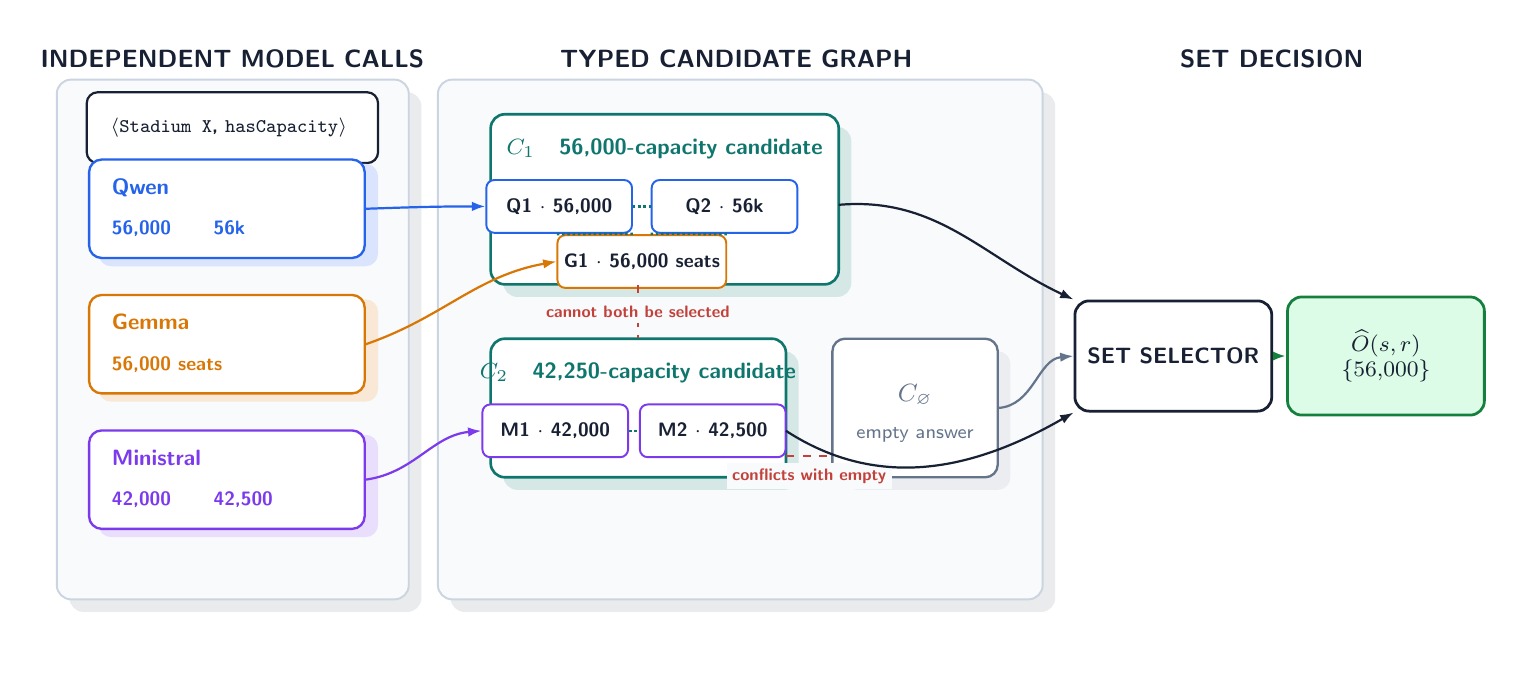
\begin{tikzpicture}[x=1cm,y=1cm]

\path[fill=white] (-0.15,-0.15) rectangle (18.45,7.95);

\node[stage] at (2.45,7.55) {INDEPENDENT MODEL CALLS};
\node[stage] at (8.85,7.55) {TYPED CANDIDATE GRAPH};
\node[stage] at (15.65,7.55) {SET DECISION};

% ---------------------------------------------------------------------------
% Left: one query, three independent parametric memories.
% ---------------------------------------------------------------------------
\path[fill=ink!9,rounded corners=1.8mm] (0.38,0.53) rectangle (4.85,7.13);
\path[fill=plane,draw=planeedge,line width=0.7pt,rounded corners=1.8mm]
  (0.22,0.69) rectangle (4.69,7.29);

\node[
  rounded corners=1.4mm,
  draw=ink,
  fill=white,
  line width=0.8pt,
  minimum width=37mm,
  minimum height=9mm,
  font=\sffamily\bfseries\fontsize{7.5}{8.6}\selectfont
] at (2.45,6.68) {
  \(\langle\)\texttt{Stadium X}, \texttt{hasCapacity}\(\rangle\)
};

% Shadows behind model calls.
\path[fill=qwen!17,rounded corners=1.6mm] (0.75,4.92) rectangle (4.30,6.22);
\path[fill=gemma!17,rounded corners=1.6mm] (0.75,3.20) rectangle (4.30,4.50);
\path[fill=ministral!17,rounded corners=1.6mm] (0.75,1.48) rectangle (4.30,2.78);

\node[model,draw=qwen] (qwenbox) at (2.38,5.65) {};
\node[
  anchor=north west,
  text=qwen,
  font=\sffamily\bfseries\fontsize{8}{9}\selectfont
] at ($(qwenbox.north west)+(1.8mm,-1.4mm)$) {Qwen};
\node[
  anchor=south west,
  text=qwen,
  font=\sffamily\bfseries\fontsize{6.7}{7.5}\selectfont
] at ($(qwenbox.south west)+(1.8mm,1.6mm)$) {56,000\qquad 56k};

\node[model,draw=gemma] (gemmabox) at (2.38,3.93) {};
\node[
  anchor=north west,
  text=gemma,
  font=\sffamily\bfseries\fontsize{8}{9}\selectfont
] at ($(gemmabox.north west)+(1.8mm,-1.4mm)$) {Gemma};
\node[
  anchor=south west,
  text=gemma,
  font=\sffamily\bfseries\fontsize{6.7}{7.5}\selectfont
] at ($(gemmabox.south west)+(1.8mm,1.6mm)$) {56,000 seats};

\node[model,draw=ministral] (ministralbox) at (2.38,2.21) {};
\node[
  anchor=north west,
  text=ministral,
  font=\sffamily\bfseries\fontsize{8}{9}\selectfont
] at ($(ministralbox.north west)+(1.8mm,-1.4mm)$) {Ministral};
\node[
  anchor=south west,
  text=ministral,
  font=\sffamily\bfseries\fontsize{6.7}{7.5}\selectfont
] at ($(ministralbox.south west)+(1.8mm,1.6mm)$) {42,000\qquad 42,500};

% ---------------------------------------------------------------------------
% Middle: concrete surface nodes grouped into typed components.
% ---------------------------------------------------------------------------
\path[fill=ink!9,rounded corners=1.8mm] (5.22,0.53) rectangle (12.90,7.13);
\path[fill=plane,draw=planeedge,line width=0.7pt,rounded corners=1.8mm]
  (5.06,0.69) rectangle (12.74,7.29);

% Component C1: Qwen and Gemma surfaces normalize to one numeric hypothesis.
\path[fill=graph!17,rounded corners=1.8mm] (5.89,4.53) rectangle (10.31,6.69);
\path[
  fill=white,
  draw=graph,
  line width=0.95pt,
  rounded corners=1.8mm
] (5.73,4.69) rectangle (10.15,6.85);

\node[
  anchor=north,
  text=graph,
  font=\sffamily\bfseries\fontsize{8}{9}\selectfont
] at (7.94,6.66) {\(C_1\)\quad 56,000-capacity candidate};

\node[raw,draw=qwen] (q1) at (6.60,5.68) {Q1 \(\cdot\) 56,000};

\node[raw,draw=qwen] (q2) at (8.70,5.68) {Q2 \(\cdot\) 56k};

\node[raw,draw=gemma] (g1) at (7.65,4.98) {G1 \(\cdot\) 56,000 seats};

\draw[draw=graph,line width=0.9pt,densely dotted] (q1.east) -- (q2.west);
\draw[draw=graph,line width=0.9pt,densely dotted]
  (q1.south east) -- (g1.north west);
\draw[draw=graph,line width=0.9pt,densely dotted]
  (q2.south west) -- (g1.north east);

% Component C2: a distinct Ministral-supported hypothesis.
\path[fill=graph!17,rounded corners=1.8mm] (5.89,2.08) rectangle (9.64,3.84);
\path[
  fill=white,
  draw=graph,
  line width=0.95pt,
  rounded corners=1.8mm
] (5.73,2.24) rectangle (9.48,4.00);

\node[
  anchor=north,
  text=graph,
  font=\sffamily\bfseries\fontsize{8}{9}\selectfont
] at (7.60,3.82) {\(C_2\)\quad 42,250-capacity candidate};

\node[raw,draw=ministral] (m1) at (6.55,2.83) {M1 \(\cdot\) 42,000};

\node[raw,draw=ministral] (m2) at (8.55,2.83) {M2 \(\cdot\) 42,500};

\draw[draw=graph,line width=0.9pt,densely dotted] (m1.east) -- (m2.west);

% Explicit empty-answer hypothesis.
\path[fill=muted!13,rounded corners=1.6mm] (10.23,2.08) rectangle (12.33,3.84);
\path[
  fill=white,
  draw=muted,
  line width=0.85pt,
  rounded corners=1.6mm
] (10.07,2.24) rectangle (12.17,4.00);
\node[
  text=muted,
  font=\sffamily\bfseries\fontsize{9}{10}\selectfont
] (null) at (11.12,3.28) {\(C_{\varnothing}\)};
\node[text=muted] at (11.12,2.78) {empty answer};

% Each model contributes only to its own generated surfaces/components.
\draw[flow,draw=qwen] (qwenbox.east) to[out=2,in=180] (q1.west);
\draw[flow,draw=gemma] (gemmabox.east) to[out=19,in=190] (g1.west);
\draw[flow,draw=ministral] (ministralbox.east) to[out=8,in=185] (m1.west);

% Typed component relations for this single-valued numeric query.
\draw[
  draw=conflict,
  line width=0.85pt,
  dashed
] (7.60,4.68) -- node[
  fill=plane,
  text=conflict,
  inner sep=0.7mm,
  font=\sffamily\bfseries\fontsize{6.5}{7.3}\selectfont
] {cannot both be selected} (7.60,4.01);

\draw[
  draw=conflict,
  line width=0.85pt,
  dashed
] (9.48,2.51) -- node[
  fill=plane,
  text=conflict,
  inner sep=0.7mm,
  font=\sffamily\bfseries\fontsize{6.5}{7.3}\selectfont,
  anchor=north,
  yshift=-0.8mm
] {conflicts with empty} (10.07,2.51);

% ---------------------------------------------------------------------------
% Right: one simple set selector and a concrete answer.
% ---------------------------------------------------------------------------
\node[
  rounded corners=1.8mm,
  draw=ink,
  fill=white,
  line width=1pt,
  minimum width=25mm,
  minimum height=14mm,
  font=\sffamily\bfseries\fontsize{8.5}{9.7}\selectfont
] (selector) at (14.40,3.78) {SET SELECTOR};

\node[
  rounded corners=1.8mm,
  draw=success,
  fill=successlight,
  line width=1pt,
  minimum width=25mm,
  minimum height=15mm,
  font=\sffamily\bfseries\fontsize{8.3}{9.4}\selectfont
] (answer) at (17.10,3.78) {
  \(\widehat{O}(s,r)\)\\[-0.2mm]
  \(\{56{,}000\}\)
};

\draw[flow,draw=ink] (10.15,5.70) to[out=5,in=155] (selector.north west);
\draw[flow,draw=ink] (9.48,2.83) to[out=-33,in=210] (selector.south west);
\draw[flow,draw=muted] (12.17,3.12) to[out=3,in=185] (selector.west);
\draw[flow,draw=success,line width=1pt] (selector.east) -- (answer.west);

\end{tikzpicture}
\end{document}
